\let\negmedspace\undefined
\let\negthickspace\undefined
\documentclass[journal,12pt,twocolumn]{IEEEtran}

\usepackage{cite}
\usepackage{amsmath,amssymb,amsfonts,amsthm}
\usepackage{algorithmic}
\usepackage{graphicx}
\usepackage{textcomp}
\usepackage{xcolor}
\usepackage{txfonts}
\usepackage{listings}
\usepackage{enumitem}
\usepackage{mathtools}
\usepackage{gensymb}
\usepackage[breaklinks=true]{hyperref}
\usepackage{tkz-euclide} % loads  TikZ and tkz-base
\usepackage{listings}
\usepackage{circuitikz}
\usepackage{graphicx}

%\newcounter{MYtempeqncnt}
\DeclareMathOperator*{\Res}{Res}
%\renewcommand{\baselinestretch}{2}
\renewcommand\thesection{\arabic{section}}
\renewcommand\thesubsection{\thesection.\arabic{subsection}}
\renewcommand\thesubsubsection{\thesubsection.\arabic{subsubsection}}

\renewcommand\thesectiondis{\arabic{section}}
\renewcommand\thesubsectiondis{\thesectiondis.\arabic{subsection}}
\renewcommand\thesubsubsectiondis{\thesubsectiondis.\arabic{subsubsection}}

% correct bad hyphenation here
\hyphenation{op-tical net-works semi-conduc-tor}
\def\inputGnumericTable{}                                 %%

\lstset{
	frame=single,
	breaklines=true,
	columns=fullflexible
}

\newtheorem{theorem}{Theorem}[section]
\newtheorem{problem}{Problem}
\newtheorem{proposition}{Proposition}[section]
\newtheorem{lemma}{Lemma}[section]
\newtheorem{corollary}[theorem]{Corollary}
\newtheorem{example}{Example}[section]
\newtheorem{definition}[problem]{Definition}
\newcommand{\BEQA}{\begin{eqnarray}}
	\newcommand{\EEQA}{\end{eqnarray}}
\newcommand{\define}{\stackrel{\triangle}{=}}
\newcommand\figref{Fig.~\ref}
\newcommand\tabref{Table~\ref}
\bibliographystyle{IEEEtran}
%\bibliographystyle{ieeetr}


\providecommand{\mbf}{\mathbf}
\providecommand{\pr}[1]{\ensuremath{\Pr\left(#1\right)}}
\providecommand{\qfunc}[1]{\ensuremath{Q\left(#1\right)}}
\providecommand{\sbrak}[1]{\ensuremath{{}\left[#1\right]}}
\providecommand{\lsbrak}[1]{\ensuremath{{}\left[#1\right.}}
\providecommand{\rsbrak}[1]{\ensuremath{{}\left.#1\right]}}
\providecommand{\brak}[1]{\ensuremath{\left(#1\right)}}
\providecommand{\lbrak}[1]{\ensuremath{\left(#1\right.}}
\providecommand{\rbrak}[1]{\ensuremath{\left.#1\right)}}
\providecommand{\cbrak}[1]{\ensuremath{\left\{#1\right\}}}
\providecommand{\lcbrak}[1]{\ensuremath{\left\{#1\right.}}
\providecommand{\rcbrak}[1]{\ensuremath{\left.#1\right\}}}
\theoremstyle{remark}
\newtheorem{rem}{Remark}
\newcommand{\sgn}{\mathop{\mathrm{sgn}}}
\providecommand{\abs}[1]{\left\vert#1\right\vert}
\providecommand{\res}[1]{\Res\displaylimits_{#1}}
\providecommand{\norm}[1]{\left\lVert#1\right\rVert}
%\providecommand{\norm}[1]{\lVert#1\rVert}
\providecommand{\mtx}[1]{\mathbf{#1}}
\providecommand{\mean}[1]{E\left[ #1 \right]}
\providecommand{\fourier}{\overset{\mathcal{F}}{ \rightleftharpoons}}
%\providecommand{\hilbert}{\overset{\mathcal{H}}{ \rightleftharpoons}}
\providecommand{\system}{\overset{\mathcal{H}}{ \longleftrightarrow}}
%\newcommand{\solution}[2]{\textbf{Solution:}{#1}}
\newcommand{\solution}{\noindent \textbf{Solution: }}
\newcommand{\cosec}{\,\text{cosec}\,}
\providecommand{\dec}[2]{\ensuremath{\overset{#1}{\underset{#2}{\gtrless}}}}
\newcommand{\myvec}[1]{\ensuremath{\begin{pmatrix}#1\end{pmatrix}}}
\newcommand{\mydet}[1]{\ensuremath{\begin{vmatrix}#1\end{vmatrix}}}
\renewcommand{\abstractname}{Question}

\let\vec\mathbf

\vspace{3cm}


\newcommand{\permcomb}[4][0mu]{{{}^{#3}\mkern#1#2_{#4}}}
\newcommand{\comb}[1][-1mu]{\permcomb[#1]{C}}

%\IEEEpeerreviewmaketitle

\newcommand \tab [1][1cm]{\hspace*{#1}}
%\newcommand{\Var}{$\sigma ^2$}
\usepackage{amssymb}
\usepackage{amsmath}
\title{
	
	\title{NCERT Maths 10.5.3 Q14}
	\author{EE23BTECH11201 - ABBURI TANUSHA$^{*}$% <-this % stops a space
	}
	
	
}
\begin{document}
\maketitle
	
\textbf{Question:} 
Find the sum of odd numbers between $0$ and $50$.

\solution
\begin{table}[h!]
	\centering
	 \resizebox{6cm}{!}{
	 	\begin{table}[H]
    \centering
    \renewcommand\thetable{1}
    \setlength{\extrarowheight}{9pt}
    \resizebox{0.51\textwidth}{!}{
    \begin{tabular}{|c|c|c|}
    \hline
    \textbf{$r\brak{i}$} & \textbf{$p\brak{i}$} & \textbf{$k\brak{i}$} \\ \hline
    $0.06029142-0.14682007jj$ &0.88475217+0.0445749j&$2.19006287\times10^{-5}$  \\ \hline
    $0.06029142+0.14682007jj$ &0.88475217-0.0445749j&$-$  \\ \hline
    $-0.06029459+0.02518904j$ &0.94427798+0.11485352jj&$-$  \\ \hline
    $-0.06029459-0.02518904j$ & 0.94427798-0.11485352j&$-$  \\ \hline
    \end{tabular}}
    \caption{Values of $ r(i) , p(i) , k(i)$}
    \label{tab:values of r(i) , p(i) , k(i)}
    \end{table}

	 	}
	 	\caption{Given Parameters}
	 	\label{tab:my_label}
 \end{table}

Last term of the given sequence is 49.
\begin{align}
 \therefore ( 2n +1 ) &= 49 \\
 2n &= 48 \\
\implies n &= 24 
\end{align}
Applying Z transform:
From equation \eqref{eq:11.9.5.26.2}:  
\begin{align}
    &= \frac{1+z^{-1}}{(1-z^{-1})^2},  \quad \abs{z} > \abs{1}  
\end{align}
For AP, the sum of first n+1 terms can be written as :
\begin{align}
	 y(n)&=x(n)*u(n) \\
	Y(z) &= X(z)U(z)\\
	&=\frac{1}{(1-z^{-1})^2} + \frac{2z^{-1}}{(1-z^{-1})^3}, \quad \abs{z} > \abs{1} 
\end{align}
Using contour integration to find inverse Z transform:
\begin{align}
	y(n) &= \frac{1}{2\pi j} \oint_C Y(z) z^{n-1} dz\\
	&= \frac{1}{2\pi j} \oint_C \brak{ \frac{1}{(1-z^{-1})^2} + \frac{2z^{-1}}{(1-z^{-1})^3} }z^{n-1} \, dz
\end{align}
The sum of the terms of the sequence is computed using the residue theorem, expressed as $R_i$, which represents the residue of the Z-transform at $ z=1 $ for the expression $ Y(z) $.
\begin{align}
	R_i=R_1 + R_2
\end{align}
 $R_1$ and $R_2$ are residues calculated at the poles of the Z-transform.
\begin{align}
		R_1 &= \frac{1}{{(2-1)!}} \frac{d (z^{25})}{dz} |_{z=1} \\	
		&= 25 
\end{align}
\begin{align}
	R_2 &= \frac{1}{{(3-1)!}}  \frac{d^2(2z^{25})}{dz^2} |_{z=1} \\
	&= 25 \times 24 \\
	&= 600 
\end{align}
\begin{align}
 R_i  &= 600 + 25\\ 
   \end{align}
   Sum of the numbers is $R_i$ = 625.
   \begin{figure}[h!]
	\centering
	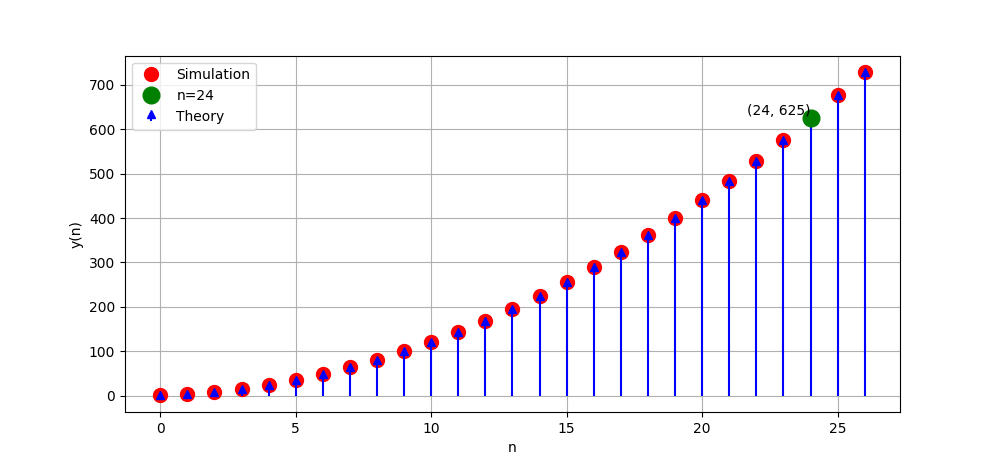
\includegraphics[width=\columnwidth]{figs/stem_plot.png}
	\label{fig:plot}
\end{figure}
\end{document}

 
